\documentclass[11pt,a4paper]{article}

% --- packages (all standard TeX Live) ---
\usepackage{lmodern}
\usepackage[T1]{fontenc}
\usepackage[utf8]{inputenc}
\usepackage[margin=2.4cm]{geometry}
\usepackage{amsmath,amssymb}
\usepackage{booktabs}
\usepackage{array}
\usepackage{xcolor}
\usepackage{enumitem}
\usepackage{graphicx}
\usepackage{tikz}
\usetikzlibrary{positioning,arrows.meta,shapes.geometric,fit,backgrounds,calc}
\usepackage[hidelinks]{hyperref}

% allow TeX a little slack so long \texttt tokens don't overflow the margin
\emergencystretch=3em

% --- convenience macros ---
\newcommand{\betau}{\ensuremath{\mathrm{sr^{-1}\,m^{-1}}}}
\newcommand{\degc}{\ensuremath{^\circ\mathrm{C}}}
\newcommand{\Tzero}{\ensuremath{T_0}}
\newcommand{\code}[1]{\texttt{#1}}
\newcommand{\target}[1]{\textsc{#1}}

\title{\textbf{ceiloclass}: radar-free target classification\\
from a single ceilometer and a model temperature field}
\author{Cloudnet / FMI}
\date{\today}

\begin{document}
\maketitle

\begin{abstract}
\noindent
\code{ceiloclass} classifies atmospheric targets --- cloud droplets, supercooled
liquid, ice, drizzle/rain and aerosol --- from a \emph{single} ceilometer or
lidar (attenuated backscatter, plus depolarization on the Vaisala CL61) together
with a Cloudnet numerical-weather-model temperature field. It carries \emph{no}
cloud radar, and is a port of the radar-free parts of CloudnetPy's categorize and
target-classification code. The pipeline is one-directional:
\textbf{read $\rightarrow$ model $\rightarrow$ detect $\rightarrow$ classify
$\rightarrow$ plot}. This paper documents each step, the physical reasoning
behind it, and --- importantly --- the places where the implementation
\emph{deliberately diverges} from CloudnetPy to compensate for the missing radar.
The three principal divergences are a data-adaptive backscatter threshold, a
top-most freezing-level crossing, and (on the CL61) the use of depolarization to
anchor the ice/rain boundary to observed ice rather than to the raw model
\Tzero{} level.
\end{abstract}

\tableofcontents
\medskip
\hrule

%======================================================================
\section{Introduction}
%======================================================================

A ceilometer measures range-corrected attenuated backscatter $\beta(t, z)$ as a
function of time $t$ and range $z$. Unlike a cloud radar it cannot, on its own,
separate hydrometeor phase: a bright backscatter return may be a liquid droplet
cloud, falling ice, or dense aerosol. CloudnetPy resolves this ambiguity by
combining lidar with radar reflectivity, Doppler velocity and
linear depolarization. \code{ceiloclass} reconstructs as much of that
classification as possible \emph{without} the radar, leaning instead on:

\begin{enumerate}[nosep]
  \item the \textbf{model temperature field}, which fixes where the air is warm
        enough for liquid and cold enough for ice;
  \item the \textbf{shape of the backscatter profile}, which distinguishes a
        sharp liquid-droplet peak from a diffuse aerosol or ice return;
  \item \textbf{linear depolarization} on the CL61, which directly separates
        (spherical, weakly depolarizing) liquid from (non-spherical, strongly
        depolarizing) ice.
\end{enumerate}

The output is a per-pixel \target{Target} category on the ceilometer
$(\text{time}\times\text{range})$ grid. Reading and harmonizing raw instrument
data is delegated to \code{ceilopyter}, which yields a \code{Ceilo} object
exposing \code{time}, \code{range}, \code{beta} (screened backscatter, a masked
array whose mask means ``no signal'') and, when available, \code{depol}. The same
pipeline runs unchanged on anything \code{ceilopyter} reads into a \code{Ceilo}:
besides ceilometers, the harmonized PollyXT, DIAL (e.g.\ the Vaisala DA10) and
doppler-lidar products, all carrying ceilometer-scale backscatter --- only the
CL61 adds depolarization, so every other instrument takes the no-depol path.

\paragraph{Notation.}
Throughout, $\beta$ is the screened backscatter (\betau), $z$ the range above the
instrument (m), $t$ time, $T_w$ the wet-bulb temperature (K), and
$\Tzero = 273.16\,\mathrm{K}$ the freezing threshold (the triple point of water)
used everywhere as the liquid/ice temperature boundary. A boolean field over the
grid is called a \emph{mask}; ``signal'' denotes the unmasked pixels
$\neg\,\mathrm{mask}(\beta)$.

%======================================================================
\section{Pipeline overview}
%======================================================================

\begin{figure}[h]
\centering
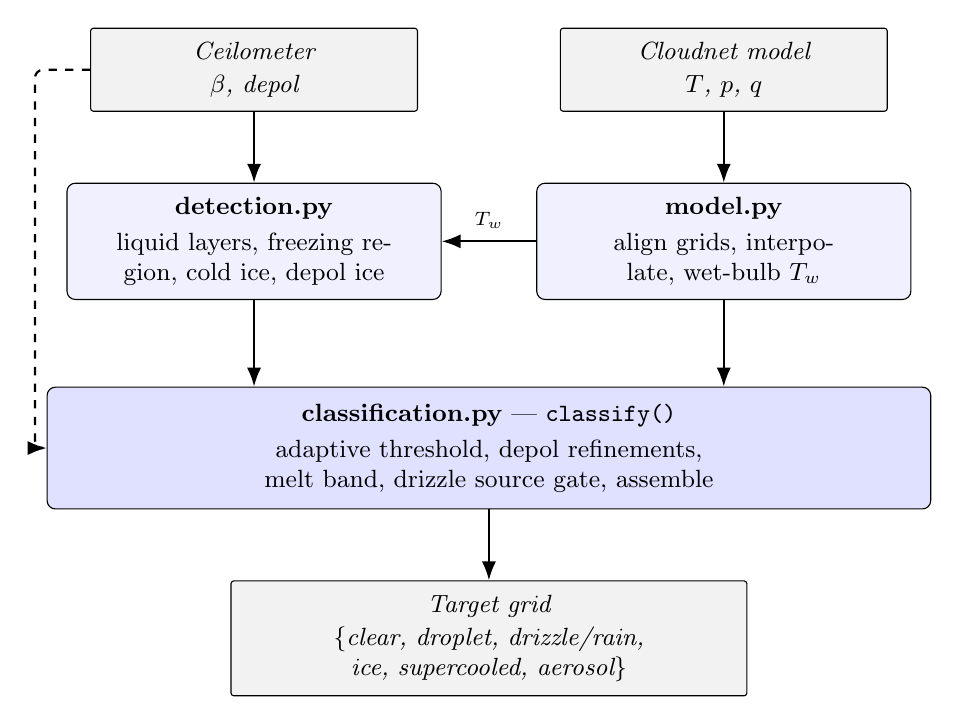
\begin{tikzpicture}[
  node distance=9mm and 18mm,
  data/.style={draw, rounded corners=1pt, align=center, inner sep=5pt,
               text width=38mm, font=\small\itshape, fill=gray!10},
  proc/.style={draw, rounded corners=3pt, align=center, inner sep=5pt,
               text width=44mm, minimum height=13mm, font=\small, fill=blue!6},
  big/.style={draw, rounded corners=3pt, align=center, inner sep=6pt,
              text width=108mm, minimum height=13mm, font=\small, fill=blue!12},
  result/.style={draw, rounded corners=1pt, align=center, inner sep=5pt,
              text width=62mm, font=\small\itshape, fill=gray!10},
  arr/.style={-{Latex[length=2.4mm]}, thick, rounded corners=3pt},
  feed/.style={arr, dashed}
]
% inputs
\node[data] (ceilo) {Ceilometer\\[1pt] $\beta$,\ depol};
\node[data, right=of ceilo] (model) {Cloudnet model\\[1pt] $T$,\ $p$,\ $q$};
% processing column
\node[proc, below=of ceilo] (detect) {\textbf{detection.py}\\[2pt]
  liquid layers, freezing region, cold ice, depol ice};
\node[proc, below=of model] (mod) {\textbf{model.py}\\[2pt]
  align grids, interpolate, wet-bulb $T_w$};
% orchestrator, spanning both columns
\node[big, below=11mm of $(detect.south)!0.5!(mod.south)$, anchor=north] (classify)
  {\textbf{classification.py}\ ---\ \code{classify()}\\[2pt]
   adaptive threshold, depol refinements,\\
   melt band, drizzle source gate, assemble};
% output
\node[result, below=of classify] (output)
  {Target grid\\[1pt] \{clear, droplet, drizzle/rain, ice, supercooled, aerosol\}};

% vertical data flow
\draw[arr] (ceilo) -- (detect);
\draw[arr] (model) -- (mod);
\draw[arr] (detect.south) -- (detect.south |- classify.north);
\draw[arr] (mod.south)    -- (mod.south    |- classify.north);
\draw[arr] (classify) -- (output);
% model temperature also feeds the temperature-based detection masks
% (freezing region, cold ice, supercooled limit)
\draw[arr] (mod.west) -- node[above=1pt, font=\scriptsize]{$T_w$} (detect.east);
% raw beta/depol used directly by classify, routed down a clear left lane
\draw[feed] (ceilo.west) -- ++(-7mm,0) |- (classify.west);
\end{tikzpicture}
\caption{Data flow. Solid arrows are the main pipeline; the dashed feed marks the
raw backscatter/depolarization that \code{classify} also consumes directly (for
the adaptive threshold and the depol refinements), not only via
\code{detection.py}. The model wet-bulb temperature $T_w$ also feeds the
temperature-based detection masks (the freezing region, cold ice and the
supercooled limit), so several \code{detection.py} primitives depend on the model,
not on the lidar alone. Detection primitives are pure boolean masks; \code{classify}
orchestrates them into the final category grid.}
\label{fig:pipeline}
\end{figure}

The modules map onto the stages of Figure~\ref{fig:pipeline}:
\begin{description}[style=nextline, leftmargin=1.2em, nosep]
  \item[\code{model.py}] reads the model file, aligns and interpolates it onto
        the ceilometer grid, and computes wet-bulb temperature
        (Section~\ref{sec:model}).
  \item[\code{detection.py}] pure detection primitives, each a boolean mask
        (Section~\ref{sec:detect}).
  \item[\code{classification.py}] the \code{classify} orchestration, the adaptive
        backscatter threshold and the CL61 depolarization refinements
        (Sections~\ref{sec:threshold}--\ref{sec:classify}).
  \item[\code{\_interp.py}] numpy-only interpolation/peak helpers.
  \item[\code{download.py}, \code{plot.py}] Cloudnet portal fetching and curtain
        plotting (not described here).
\end{description}

%======================================================================
\section{Model temperature processing}
\label{sec:model}
%======================================================================

The model supplies temperature, pressure and specific humidity on a coarse grid
in time and height. Before these fields can inform the classification they must be
brought onto the ceilometer's own grid, and the temperature must be converted to
the wet-bulb temperature that governs the freezing level. Three considerations
shape this step: the two instruments measure height from different reference
surfaces, the interpolation must remain sensible near the ground, and the wet-bulb
conversion is nonlinear and so must follow the interpolation rather than precede
it.

\subsection{Grid alignment in absolute coordinates}

The model reports height above the surface of its grid cell, while the ceilometer
reports range above the instrument. In flat terrain the distinction is negligible,
but where the model's representation of the surface departs from the true site
altitude the two references can differ by hundreds of metres --- around 270\,m at
Granada, for example. Using the known site altitude and the model's own surface
altitude at each time step, both grids are shifted onto a common above-sea-level
datum before interpolation, so that a given model temperature is placed at the
height where the ceilometer actually samples it. Where either altitude is
unavailable the correction is omitted and both grids are treated as height above
ground, as CloudnetPy does.

\subsection{Interpolation and wet-bulb temperature}

Each model profile is interpolated onto the observation range and then along time.
The vertical interpolation extrapolates beyond the model levels rather than
holding the edge value fixed, so a site sitting below the lowest model level still
receives a physically reasonable near-ground temperature; the temporal
interpolation is clamped at the edges of the model's coverage.

The wet-bulb temperature is then derived from the already-interpolated
temperature, pressure and humidity. This ordering follows CloudnetPy and matters
because the wet-bulb temperature is nonlinear in its inputs: computing it on the
coarse model grid and interpolating the result would not reproduce the wet-bulb
temperature of the interpolated fields. Where the necessary thermodynamic library
is unavailable the code falls back to the dry-bulb temperature. Occasionally a
model time step carries no valid data; rather than abandoning the whole
classification, such a step is dropped and bridged by the surrounding profiles in
time.

\subsection{The extrapolated (quality) flag}

The interpolated model carries a flag marking pixels whose wet-bulb temperature
was extrapolated above the top of the model or outside its temporal coverage,
where confidence is correspondingly lower. Extrapolation below the lowest model
level is deliberately not flagged: in complex terrain a site can lie beneath the
model surface, and the downward extrapolation there is trustworthy. This flag is
passed through to the classification as its quality field.

\subsection{The freezing level \texorpdfstring{$\Tzero$}{T0}}
\label{sec:t0}

The single most important quantity derived from the model is the altitude of the
$0\,\degc$ isotherm, obtained by linear interpolation between the two adjacent
gates whose wet-bulb temperatures straddle \Tzero{}. Everything above this altitude
is the \emph{freezing region}: the domain in which ice and supercooled liquid can
occur.

Which crossing to take, when the temperature profile passes through freezing more
than once, is a deliberate departure from CloudnetPy, which always selects the
lowest crossing. On a normal day with a warm surface \code{ceiloclass} likewise
takes the lowest crossing, so that the freezing level tracks the melting layer
smoothly even when warm and cold layers alternate aloft. But when the surface
itself is below freezing --- a winter surface inversion --- it takes the topmost
crossing instead. The lowest crossing would otherwise sit at the ground and
mislabel the entire warm layer above the inversion as ice.

%======================================================================
\section{Detection primitives}
\label{sec:detect}
%======================================================================

The detection stage reduces the observations to a small set of physically
motivated masks --- liquid layers, the freezing region, cold elevated ice, and (on
the CL61) depolarization ice --- each ported from CloudnetPy and stripped to what a
lidar alone can support. The classifier of Section~\ref{sec:classify} then
composes these masks into the final categories. This section describes what each
mask captures and the physical reasoning behind it.

\subsection{Liquid droplet layers}
\label{sec:liquid}

A liquid cloud base has a characteristic backscatter signature: the return rises
to a sharp peak and then falls away steeply above it, because the lidar is
extinguished within a few tens of metres of entering the dense droplets. Liquid
layers are found by locating such peaks along each profile and testing the shape
around them. A candidate is accepted only if the peak is sufficiently bright
(exceeding $10^{-6}\,\betau$), the layer is compact (thinner than
$250\,\mathrm{m}$ and a few gates deep), it sits at least $100\,\mathrm{m}$ above
the lowest gate, and the backscatter falls off sharply enough above the peak. The
procedure follows CloudnetPy's liquid detection with the liquid-water-path and
radar top-correction steps removed, since neither a radiometer nor a radar is
available.

Two refinements extend this beyond CloudnetPy. The first concerns fog and very low
stratus. A strict local maximum cannot be found within a few gates of the profile
edge, so the lowest several gates form a blind zone in which ground-hugging liquid
would be missed and left as aerosol. A dedicated surface pass therefore takes the
strongest return in this zone, anchors its base at the ground, and applies the
same shape test with the minimum-altitude requirement relaxed, since fog by
definition sits on the surface.

The second refinement guards against dragging a liquid base down into haze.
Because the base search follows the backscatter gradient, on a hazy day it can
slide well below the cloud into the gradual sub-cloud aerosol; and because the
peak-detection amplitude lies far below the cloud/aerosol threshold of
Section~\ref{sec:threshold}, a weak bump entirely within the aerosol could even be
accepted as liquid. The base is therefore raised to the lowest gate that reaches
cloud strength, and a candidate that never reaches cloud strength at all is
rejected. The bright cloud core is kept while the sub-cloud haze reverts to
aerosol; the halo recovery of Section~\ref{sec:grow} still runs afterwards to
restore the layer's true extent.

\subsection{Cold elevated signal (falling ice)}
\label{sec:falling}

Backscatter present in sufficiently cold air is taken to be ice. This is the
lidar-only remnant of CloudnetPy's falling-hydrometeor detection: a pixel is
treated as falling ice when it carries signal, lies well above the boundary layer
(above $2000\,\mathrm{m}$), and is colder than $-15\,\degc$. Higher still, an
isolated single gate with no neighbours is discarded, so that a stray speck of
thin aerosol is not mistaken for cirrus.

\subsection{Depolarization ice (CL61 only)}
\label{sec:depolice}

On the CL61 the linear depolarization ratio supplies directly what CloudnetPy
would otherwise take from radar. Spherical liquid droplets barely depolarize the
return ($\delta < 0.1$), whereas non-spherical ice crystals depolarize it strongly
($\delta \sim 0.3$--$0.5$). Any signal pixel whose depolarization exceeds $0.15$
--- a value that sits cleanly between the two populations --- is marked as ice.
This both vetoes false liquid layers, such as ice virga read as a droplet cloud,
and recovers ice that the cold-signal test of Section~\ref{sec:falling} misses
because it falls below the altitude or temperature cutoffs.

\subsection{Growing and filling liquid layers}
\label{sec:grow}

The peak-based detection marks only the sharp core of a liquid layer; the weaker
gates hugging its base and top belong to the same cloud but fall outside the shape
test. Two operations recover them. The first grows the droplet mask into adjacent
signal-bearing gates that are not blocked by ice, and does so asymmetrically:
generously upward (about $100\,\mathrm{m}$, to recover the attenuated true top that
the lidar could not see through) but only slightly downward (about
$10\,\mathrm{m}$, to avoid swallowing sub-cloud aerosol or drizzle). The second
relabels an entire contiguous run of signal as liquid when it contains a droplet
gate and is no thicker than about $100\,\mathrm{m}$; thicker runs, such as a thin
cloud sitting atop a deep aerosol column, are left untouched so that genuine
aerosol beneath the cloud is not absorbed.

\subsection{Supercooled limit}

Liquid water cannot persist below about $-38\,\degc$, so any droplet gates colder
than this are removed.

%======================================================================
\section{The adaptive backscatter threshold}
\label{sec:threshold}
%======================================================================

The pivotal decision in radar-free classification is: \emph{how bright
must signal be to count as cloud/precipitation rather than aerosol?} A
fixed threshold fails because aerosol load varies enormously by site
and day (a dusty Granada afternoon vs.\ a clean Arctic
morning). \code{\_adaptive\_strong\_beta} therefore derives the
threshold $\beta_{\mathrm{strong}}$ from the data distribution itself.
This is the second major divergence from CloudnetPy.

The cloud--aerosol backscatter threshold, $\beta_{\mathrm{strong}}$,
is derived adaptively from the observed backscatter distribution
rather than prescribed as a fixed value. This accounts for the large
day-to-day and site-to-site variability in aerosol loading (e.g. a
dusty continental boundary layer versus a clean Arctic atmosphere).

All positive backscatter values in the ceilometer profile are
histogrammed in logarithmic space between the 1st and 99.9th
percentiles using 60 bins, and the histogram is lightly smoothed with
a three-bin moving average to suppress noise. The lowest well-defined
mode is taken as the aerosol mode. This is not necessarily the
histogram maximum, since on heavily overcast days the cloud mode may
contain more samples than the aerosol population. A lower-valued mode
is therefore preferred whenever it is separated from the dominant peak
by a genuine minimum in the histogram, preventing small fluctuations
on the shoulder of a broad peak from being interpreted as independent
aerosol modes.

The threshold is then placed according to the histogram morphology. If
a second mode exists at substantially larger backscatter (more than
twice the aerosol-mode value and exceeding
$3\times10^{-6}\,\mathrm{sr^{-1}\,m^{-1}}$), it is interpreted as
cloud or precipitation, and the threshold is placed at the minimum
between the aerosol and cloud modes. Otherwise, the distribution is
treated as aerosol only (possibly with multiple aerosol layers), and
the threshold is placed on the right-hand shoulder of the aerosol
mode, where the histogram has fallen to 5\% of its peak value. When
multiple aerosol modes are present, the shoulder is referenced to the
highest aerosol mode so that elevated aerosol layers (e.g. lofted
Saharan dust) remain classified as aerosol rather than being separated
as cloud.

Finally, the threshold is bounded by both a relative limit (25 times
the aerosol-mode backscatter) and an absolute limit of
$10^{-5}\,\mathrm{sr^{-1}\,m^{-1}}$. The relative bound acts only as a
conservative fallback if neither a distinct valley nor shoulder can be
identified, whereas the absolute bound prevents unrealistically large
thresholds in cases where aerosol and cloud are not separable, such as
persistent polar low-cloud conditions. If fewer than 1000 valid
backscatter samples are available, the algorithm returns the default
threshold of $3\times10^{-6}\,\mathrm{sr^{-1}\,m^{-1}}$.

Figure~\ref{fig:adaptive_beta} illustrates four representative
histogram morphologies encountered by the adaptive threshold
algorithm, demonstrating how the threshold is placed for bimodal cloud
cases, multilayer aerosol, clean conditions, and polar-winter
low-cloud continua.

\begin{figure}[t]
\centering 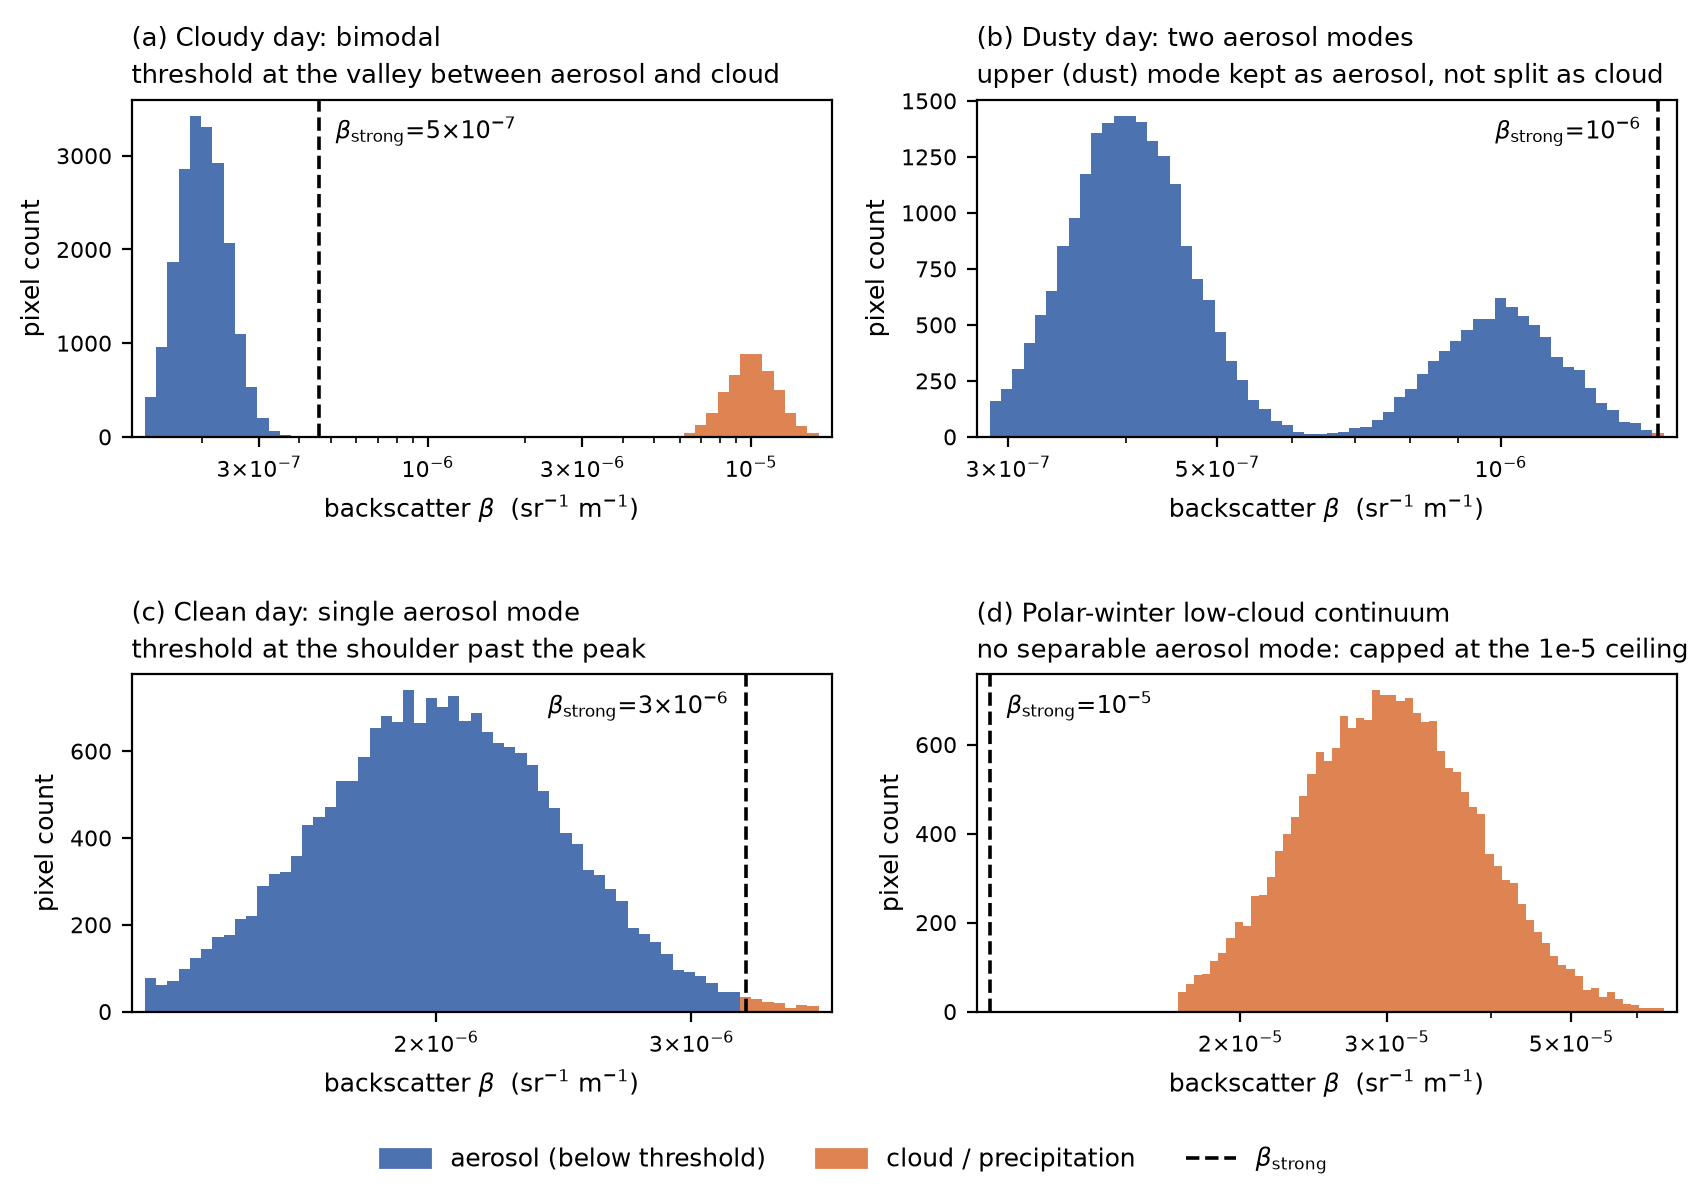
\includegraphics[width=\linewidth]{adaptive_threshold.png}
\caption{Adaptive backscatter threshold ($\beta_{\mathrm{strong}}$,
  dashed line) for four representative backscatter histograms, each
  corresponding to a ceiloclass regression case. Histogram bars are
  coloured according to the resulting classification: aerosol below
  the threshold (blue) and cloud or precipitation above (orange). The
  algorithm places the threshold (a) at the valley between aerosol and
  cloud modes, (b) above a secondary aerosol mode that does not
  satisfy the cloud-bright criterion, (c) on the shoulder of a single
  aerosol mode, and (d) at the absolute upper limit when no separable
  aerosol mode is present.}
\label{fig:adaptive_beta}
\end{figure}

%======================================================================
\section{Classification assembly}
\label{sec:classify}
%======================================================================

The classifier brings the detection masks and the model together into the final
category grid. Setting depolarization aside for the moment, its logic is
straightforward. It first establishes the freezing region
(Section~\ref{sec:t0}) and the liquid layers (Section~\ref{sec:liquid}), grows and
fills the latter and trims any that are too cold to be liquid, and selects the
cloud/aerosol threshold of Section~\ref{sec:threshold}. Signal brighter than this
threshold, once the droplet layers are set aside, is the strong non-liquid return
that marks hydrometeors: within the freezing region it is ice, and in the warm air
below it is drizzle or rain, subject to the source test of
Section~\ref{sec:source}. Any remaining signal, too weak to be a hydrometeor, is
aerosol. The categories are then assembled with a fixed precedence and the result
is despeckled (Section~\ref{sec:assemble}).

\subsection{Depolarization refinements (CL61 only)}

On the CL61 the depolarization-based ice mask of Section~\ref{sec:depolice}
sharpens three parts of this picture, each tied to the phase change at the melting
level.

\paragraph{(a) Protecting liquid from its own multiple scattering.}
Deep inside a liquid layer the depolarization climbs as photons scatter multiple
times, and left unchecked this would trip the ice veto and carve the densest part
of a real droplet cloud out into ice. Genuine liquid layers are recognized by the
low-depolarization single-scattering signature at their base, which pure ice
lacks, and are shielded from the veto --- the whole layer together with a short
tail above it, of order $80\,\mathrm{m}$, covering the observed reach of the
multiple-scattering enhancement. Where depolarization is available it also
replaces the cold-signal heuristic of Section~\ref{sec:falling} as the barrier to
upward liquid growth, so that a genuinely high supercooled cloud top --- as seen at
Troll --- is not clipped away.

\paragraph{(b) Extending the freezing region down to observed ice.}
When the model places the $0\,\degc$ level too high, depolarization-confirmed ice
--- falling ice not yet melted --- is left stranded on the warm side of the
boundary. The freezing region is then flooded downward through the connected ice
to meet this observed base, but by no more than $1500\,\mathrm{m}$, so that lofted
dust touching a cloud cannot drag the whole column below freezing. Two conditions
restrain the flood. It follows only cloud-strength signal, so that a boundary layer
full of weakly scattering but strongly depolarizing aerosol such as dust or pollen
cannot carry it to the ground; and it requires the high depolarization of solid
ice ($\delta > 0.30$, well beyond the $0.15$ ice/liquid limit), so that it stops at
the phase change itself. Across the melting level the depolarization falls from
that of solid ice to the lower value of the wet, melting particles below, and the
solid-ice base sits at this drop; keying on it prevents the freezing region from
running on down through the still-depolarizing rain beneath $0\,\degc$. The
resulting ice base is smoothed against noisy single-profile spikes by clipping it
to its rolling median over neighbouring profiles. Figure~\ref{fig:extendice} shows
a case where this applies.

\begin{figure}[t]
\centering
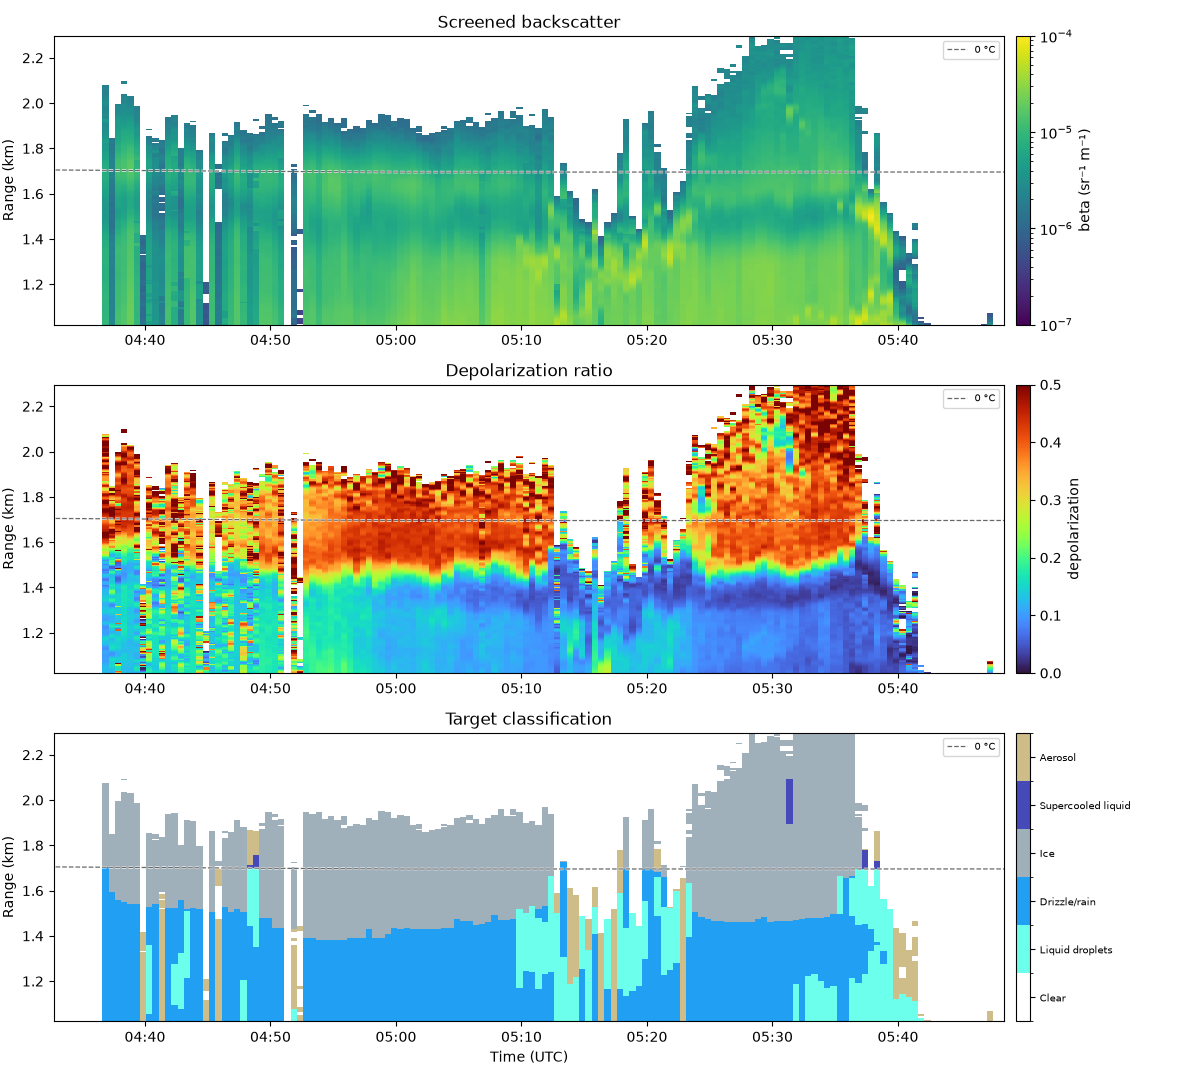
\includegraphics[width=\linewidth]{extend-ice-below-t0.png}
\caption{Extending the ice region down to observed ice on a CL61 case (panels:
screened backscatter, depolarization, target classification; dashed line is the model
$0\,\degc$ level at $\sim$1.7\,km). The depolarization panel shows cloud-strength,
strongly depolarizing ice reaching \emph{below} the model $0\,\degc$ line ---
falling ice not yet melted, where the model freezing level is biased high. The
classification extends the ice region down to that observed base rather than
mislabelling the sub-\Tzero{} ice as drizzle/rain.}
\label{fig:extendice}
\end{figure}

\paragraph{(c) The melt band: extending rain up to observed ice.}
The mirror image occurs when a depolarization-ice base sits above the model
$0\,\degc$ level: the true melting level is then higher than the model's, and the
layer between them --- cold according to the model, but cloud-strength and only
weakly depolarizing --- is ice already melting into rain. This band is identified
as the cloud-strength signal reachable both downward from the ice base and upward
from the warm air, a continuous column linking the ice down to the rain across the
melting level. Requiring both connections excludes weakly depolarizing patches
buried inside an ice cloud and supercooled layers with no ice above them. Because
the melting particles themselves depolarize, a thin high-depolarization
enhancement at the melt level (no more than $150\,\mathrm{m}$) is bridged rather
than allowed to block the connection, while a thick coherent ice cloud still blocks
it. The band is then removed from the freezing region so that it classifies as
drizzle or rain. Figure~\ref{fig:meltband} shows this on a stratiform-rain day.

There is a deliberate asymmetry between (b) and (c). The downward extension keys on
the solid-ice depolarization ($0.30$), whereas the melt band keys on the lower
ice/liquid value ($0.15$). Above a $0\,\degc$ level biased low the air is genuinely
warm and the melted drops are near-spherical, so the rain there depolarizes weakly;
a depolarization between $0.15$ and $0.30$ on the cold side of the boundary is
still ice and must not be stripped to rain, as a solid-ice threshold applied there
would wrongly do.

\begin{figure}[t]
\centering
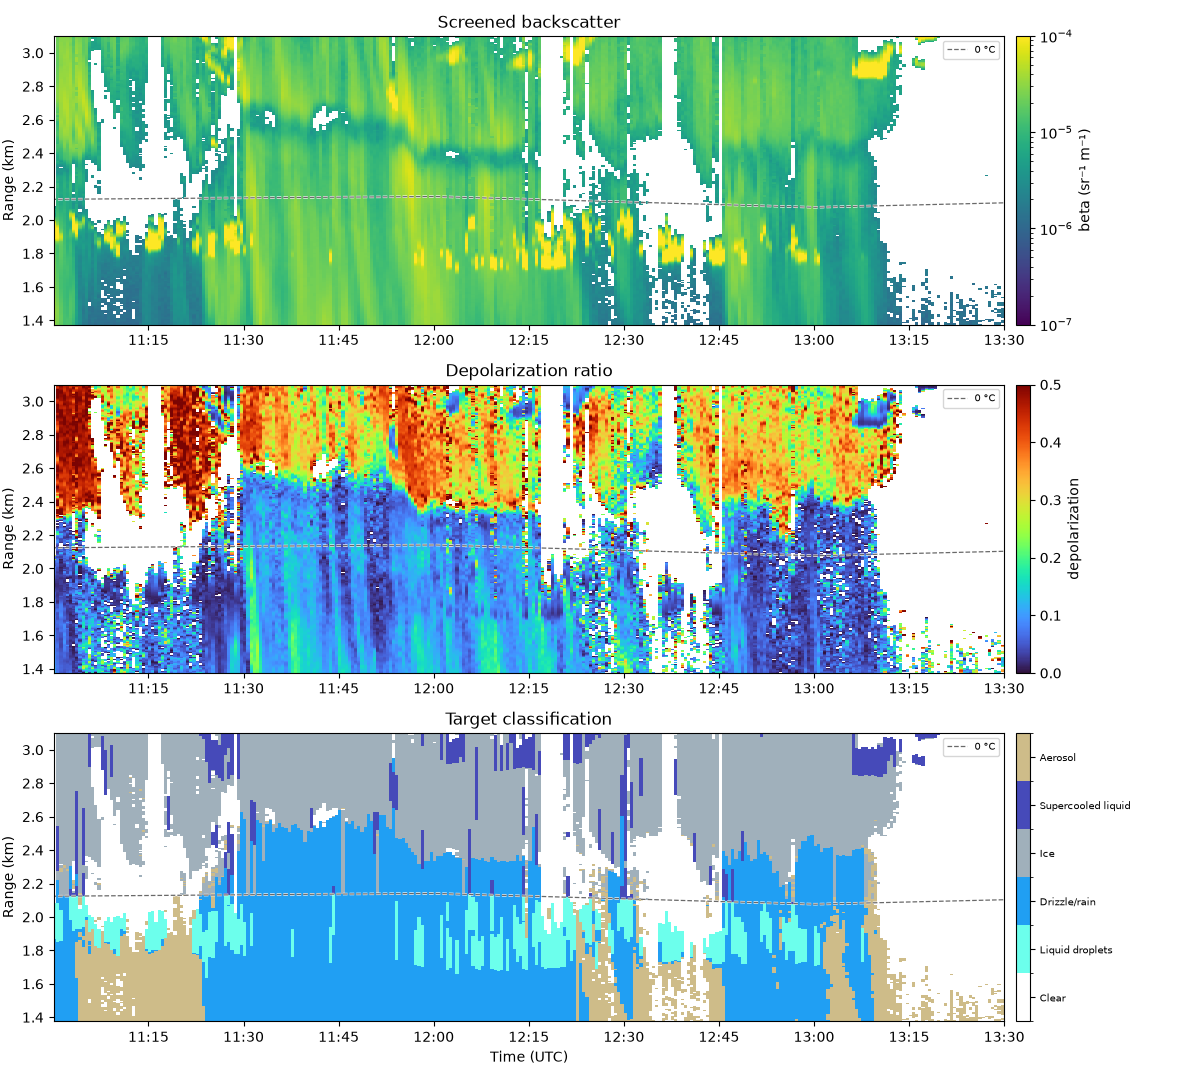
\includegraphics[width=\linewidth]{extended-drizzle-above-t0.png}
\caption{The melt band on a stratiform-rain CL61 day at
Lindenberg (panels: screened backscatter, depolarization, target classification;
dashed line is the model $0\,\degc$ level at $\sim$2.1\,km). The depol-ice base
(strong depolarization above the low-depol rain) sits \emph{above} the model
$0\,\degc$ line, so the real melt level is higher than the model's. The cold,
cloud-strength, low-depol band between $\Tzero$ and the ice base is relabelled
drizzle/rain --- the rain extends above the model $0\,\degc$ line up to the
observed melt level.}
\label{fig:meltband}
\end{figure}

\subsection{The drizzle source gate}
\label{sec:source}

Drizzle and rain fall from a cloud: precipitation and the cloud that produces it
form a single continuous column of signal. A warm bright gate is therefore kept as
drizzle or rain only when a cloud --- a liquid layer or ice --- lies above it with
unbroken signal in between. This rejects two kinds of false precipitation: a bright
layer cut off from anything above by clear air, such as a near-surface aerosol blob
far below an unrelated cirrus; and a bright layer whose only nearby cloud lies
below rather than above it, such as haze resting on a shallow surface fog. The
latter is what keeps the bright, cloud-free marine haze at Mindelo classified as
aerosol rather than drizzle. To keep a ragged cloud edge from dropping a genuine
drizzle shaft beside it, the cloud mask may optionally be dilated by a few profiles
in time before the test.

\paragraph{Bridging the melting-layer notch.}
Demanding strictly unbroken signal fails at the melting level, where the
backscatter dips into a notch that often falls below the screening threshold. This
leaves a thin masked gap between the rain below and the ice above, and a single
masked gate is enough to sever the column and let the whole drizzle shaft beneath
fall through to aerosol. The source test therefore bridges a clear-air gap of up to
$100\,\mathrm{m}$, bounded by signal on both sides, before tracing the path. The
width of the gap is what distinguishes the two situations the bare continuity test
could not: a melt notch is tens of metres deep, whereas the clear air beneath an
unrelated cirrus is kilometres deep and stays unbridged. On the stratiform-rain
CL61 day at Lindenberg this recovers several thousand gates from aerosol to
drizzle, of which $98\%$ are confirmed as precipitation or melting by the
co-located radar in the standard Cloudnet product.

\subsection{Category precedence and despeckling}
\label{sec:assemble}

The categories are written in order of increasing precedence, so that later rules
overwrite earlier ones and the rule ``liquid layers sit on top'' is honoured:
%
\begin{center}
\small
aerosol $\rightarrow$ ice $\rightarrow$ drizzle/rain $\rightarrow$
droplet (warm) $\rightarrow$ supercooled (droplet $\wedge$ cold).
\end{center}
%
Finally, isolated specks left by screening noise are removed: any classified pixel
with too few classified neighbours in its immediate surroundings is cleared.

%======================================================================
\section{Output categories}
%======================================================================

\begin{table}[h]
\centering
\small
\begin{tabular}{@{}c l l@{}}
\toprule
Code & Category & Definition \\
\midrule
0 & \target{Clear}          & No signal, or speckle removed. \\
1 & \target{Droplet}        & Liquid layer in warm air ($T_w \ge \Tzero$). \\
2 & \target{Drizzle/Rain}   & Strong warm signal sourced from a cloud above. \\
3 & \target{Ice}            & Strong (or depol-confirmed) signal in cold air. \\
4 & \target{Supercooled}    & Liquid layer in cold air ($T_w < \Tzero$). \\
5 & \target{Aerosol}        & Any remaining signal below the cloud threshold. \\
\bottomrule
\end{tabular}
\caption{The \target{Target} enumeration. There is no melting class: the freezing
anchor (Sections~\ref{sec:t0} and \ref{sec:classify}) already places the ice/rain
boundary at the observed melt level.}
\end{table}

%======================================================================
\section{Summary of divergences from CloudnetPy}
%======================================================================

\begin{table}[h]
\centering
\small
\renewcommand{\arraystretch}{1.25}
\begin{tabular}{@{}p{0.27\linewidth} p{0.32\linewidth} p{0.32\linewidth}@{}}
\toprule
Aspect & CloudnetPy & \code{ceiloclass} \\
\midrule
Freezing level &
  Always the lowest \Tzero{} crossing &
  Top-most crossing under a sub-freezing surface inversion
  (Section~\ref{sec:t0}). \\
Cloud/aerosol threshold &
  Effectively fixed &
  Data-adaptive from the backscatter histogram, capped at $10^{-5}\,\betau$
  (Section~\ref{sec:threshold}). \\
Phase information &
  From cloud radar &
  From CL61 depolarization; absent for other instruments
  (Section~\ref{sec:depolice}). \\
Ice/rain boundary &
  Model melting level &
  Anchored to observed depol ice via \code{\_extend\_cold\_to\_ice} and the melt
  band (Section~\ref{sec:classify}). \\
Fog / very low stratus &
  --- &
  Dedicated surface pass into the local-maximum blind zone
  (Section~\ref{sec:liquid}). \\
\bottomrule
\end{tabular}
\caption{Where the radar-free port deliberately departs from CloudnetPy.}
\end{table}

%======================================================================
\section{Limitations}
%======================================================================

\begin{itemize}[nosep]
  \item Without radar, phase for non-CL61 instruments rests entirely on the model
        temperature and backscatter shape; the freezing region is a model
        quantity and inherits its biases (mitigated, on the CL61, by the
        depol-anchored boundary).
  \item The lidar is rapidly attenuated inside thick liquid; nothing can be said
        about cloud above an optically thick base.
  \item The adaptive threshold assumes a recognizable aerosol mode; in a
        featureless distribution it falls back to fixed defaults and caps.
  \item There is no melting-layer or insect class, and no liquid-water-path
        constraint (no radiometer).
\end{itemize}

%======================================================================
\section*{Compiling this document}
\addcontentsline{toc}{section}{Compiling this document}
%======================================================================

\begin{verbatim}
pdflatex whitepaper.tex
pdflatex whitepaper.tex   # second pass for the table of contents / refs
\end{verbatim}
\noindent
Only standard TeX Live packages are used (\code{amsmath}, \code{booktabs},
\code{tikz}, \code{hyperref}).

\end{document}
